\chapter{प्रकाशरसायन}\label{ch:b3:photochemistry}

दृष्टि तब आरंभ होती है जब एक फ़ोटॉन एक अणु को मोड़ देता है। आँख की शलाका कोशिकाओं में
रेटिनल अपने प्रोटीन में 11-सिस रूप में बैठा रहता है; हरे प्रकाश का एक फ़ोटॉन उसे
पूर्ण-ट्रांस रूप में बदल देता है, और यह समावयवन \qty{200}{fs} के भीतर लगभग पूरा हो जाता है,
जो लगभग किसी भी अन्य रासायनिक घटना से तीव्र है। दृष्टि का शेष भाग, एक विशाल जैवरासायनिक
प्रवर्धन, उसी एक मुड़े हुए अणु से आगे बढ़ता है। यही नियम (एक फ़ोटॉन एक अणु को उत्तेजित करता है,
जो फिर अनेक नियतियों में से एक चुनता है) सनस्क्रीन, तनावग्रस्त वलयों के संश्लेषण,
प्रकाशगतिक चिकित्सा, नगरों के ऊपर छाए धूम-कोहरे और उस \omterm{def:b3:photochemistry:chapman}{ओज़ोन परत} को नियंत्रित करते हैं जो
पृथ्वी के पृष्ठ को पराबैंगनी प्रकाश से बचाती है।

\begin{recall}
\Cref{ch:b3:electronic-spectroscopy} ने अणुओं की उत्तेजित अवस्थाओं, \omterm{def:b3:electronic-spectroscopy:jablonski}{याब्लोन्स्की आरेख}, \omterm{def:b3:electronic-spectroscopy:radiationless}{अंतरतंत्र संक्रमण},
\omterm{def:b3:electronic-spectroscopy:luminescence}{प्रतिदीप्ति} और \omterm{def:b3:electronic-spectroscopy:luminescence}{स्फुरदीप्ति}, शमन तथा किसी प्रकाशभौतिक प्रक्रम की \omterm{def:b3:electronic-spectroscopy:quantum-yield}{क्वांटम लब्धि} का वर्णन किया।
प्रथम वर्ष के खंड ने मूलकों, समांश विखंडन और $Z$/$E$ समावयवियों को परिभाषित किया; द्वितीय वर्ष
के खंड ने समन्वित अभिक्रियाओं, अग्रांत कक्षकों और उत्प्रेरकी चक्रों को।
\Cref{ch:b3:complex-kinetics} ने \omterm{def:b3:complex-kinetics:chain}{शृंखला अभिक्रियाओं} और स्थायी अवस्थाओं का विवेचन किया।
\end{recall}

\section{अभिकर्मक के रूप में प्रकाश}

दो पुराने सिद्धांत इस विषय का आरंभ करते हैं: केवल अवशोषित प्रकाश ही रासायनिक परिवर्तन
ला सकता है (ग्रोटहस और ड्रेपर), और प्रत्येक अवशोषित फ़ोटॉन एक अणु को उत्तेजित करता है
(स्टार्क और आइंस्टाइन)।

\begin{definition}[फ़ोटॉन फ़्लक्स, रासायनिक प्रकाशमापी]\label{def:b3:photochemistry:photon-flux}
किसी प्रकाश स्रोत का \emph{फ़ोटॉन फ़्लक्स}\index{फ़ोटॉन फ़्लक्स} वह फ़ोटॉनों की संख्या है जो वह
प्रति इकाई समय प्रदान करता है, जिसे प्रायः फ़ोटॉनों के मोल (आइंस्टाइन) प्रति सेकंड में गिना जाता है।
\emph{रासायनिक प्रकाशमापी}\index{रासायनिक प्रकाशमापी} यथार्थतः ज्ञात \omterm{def:b3:electronic-spectroscopy:quantum-yield}{क्वांटम लब्धि} वाली एक
प्रकाशरासायनिक अभिक्रिया है, जिसका उपयोग फ़ोटॉन फ़्लक्स मापने के लिए
किया जाता है।
\end{definition}

\begin{proposition}[स्टार्क--आइंस्टाइन नियम]\label{prop:b3:photochemistry:stark-einstein}
सामान्य प्रकाश तीव्रताओं पर प्रत्येक अवशोषित फ़ोटॉन ठीक एक अणु को
उत्तेजित करता है; उत्तेजित अवस्था से आरंभ होने वाले सभी प्रक्रमों की प्राथमिक \omterm{def:b3:electronic-spectroscopy:quantum-yield}{क्वांटम
लब्धियों} का योग 1 होता है।
\end{proposition}

\begin{proof}[आंशिक उपपत्ति]
कि एक समय में एक फ़ोटॉन एक अणु द्वारा अवशोषित होता है, यह स्वीकृत है (द्वि-फ़ोटॉन
अवशोषण को स्पंदित लेज़रों की तीव्रताएँ चाहिए)। उत्तेजित अणु तब दर स्थिरांकों $k_i$ वाले प्रतिस्पर्धी
प्रथम-कोटि प्रक्रमों द्वारा लुप्त होता है
(\cref{ch:b3:electronic-spectroscopy}): पथ $i$ अपनाने वाला अंश $\Phi_i =
k_i/\sum_jk_j$ है, और $\sum_i\Phi_i = 1$।
\end{proof}

किसी अभिक्रिया की \omterm{def:b3:electronic-spectroscopy:quantum-yield}{क्वांटम लब्धि}, अर्थात् प्रति अवशोषित फ़ोटॉन रूपांतरित अणुओं की संख्या,
के लिए इस सीमा का पालन आवश्यक नहीं: एक प्राथमिक प्रकाशरासायनिक चरण एक शृंखला आरंभ कर सकता है।
प्रकाश में रखा गया \ce{H2} और \ce{Cl2} का मिश्रण $10^4$ और उससे अधिक की \omterm{def:b3:electronic-spectroscopy:quantum-yield}{क्वांटम लब्धियों} के साथ
अभिक्रिया करता है, प्रत्येक प्रकाश-अपघटित \ce{Cl2} \cref{ch:b3:complex-kinetics} की
हाइड्रोजन--ब्रोमीन अभिक्रिया जैसी एक शृंखला आरंभ करता है; 1 से बड़ी \omterm{def:b3:electronic-spectroscopy:quantum-yield}{क्वांटम लब्धि}
शृंखला की पहचान है।

\begin{proposition}[प्रकाशरासायनिक अभिक्रिया की दर]\label{prop:b3:photochemistry:rate}
विकिरण तरंगदैर्ध्य पर अवशोषकता $A$ वाला एक विलयन, जो \omterm{def:b3:photochemistry:photon-flux}{फ़ोटॉन
फ़्लक्स} $I_0$ (आइंस्टाइन प्रति सेकंड) ग्रहण करता है, $I_{\mathrm{abs}} = I_0(1 - 10^{-A})$ अवशोषित करता है; यदि
अभिकारक यह सब अवशोषित करे, तो अभिक्रिया प्रति सेकंड $v = \Phi I_{\mathrm{abs}}$ मोल रूपांतरित करती है।
\end{proposition}

\begin{proof}
बियर--लैम्बर्ट नियम से पारगत फ़्लक्स $I_010^{-A}$ है, अतः अवशोषित फ़्लक्स
$I_0(1 - 10^{-A})$ है; \omterm{def:b3:electronic-spectroscopy:quantum-yield}{क्वांटम लब्धि} की परिभाषा से, प्रति अवशोषित फ़ोटॉन $\Phi$ अणु
अभिक्रिया करते हैं।
\end{proof}

\begin{method}[लैंप से प्रकाश-अभिक्रिया की दर]\label{met:b3:photochemistry:photochemical-rate}
\begin{enumerate}
  \item फ़ोटॉन ऊर्जा $E = hc/\lambda$; \omterm{def:b3:photochemistry:photon-flux}{फ़ोटॉन फ़्लक्स} $I_0 = P/E$, नमूने तक पहुँचने वाली शक्ति $P$ के लिए,
        या प्रकाशमापी से मापा हुआ; आइंस्टाइन प्रति सेकंड के लिए $N_A$ से भाग
        दीजिए।
  \item अवशोषित अंश $1 - 10^{-A}$, जहाँ $A$ विकिरण तरंगदैर्ध्य पर हो (अभिकारक के
        उपभोग के साथ यह बदलता है)।
  \item दर $\Phi I_{\mathrm{abs}}$, mol/s में; सांद्रता-दर के लिए इसे आयतन से भाग दीजिए।
\end{enumerate}
\end{method}

\begin{method}[फ़ेरीऑक्सैलेट प्रकाशमापन]\label{met:b3:photochemistry:actinometry}
\begin{enumerate}
  \item प्रयोग वाले ही सेल और ज्यामिति में, पोटैशियम ट्रिस(ऑक्सैलेटो)फ़ेरेट(III) का एक अम्लीकृत
        विलयन विकिरित कीजिए, जो इतना सांद्र हो कि लगभग \qty{450}{nm} से नीचे का
        व्यावहारिक रूप से सारा प्रकाश अवशोषित कर ले।
  \item प्रकाश एक अंशांकित \omterm{def:b3:electronic-spectroscopy:quantum-yield}{क्वांटम लब्धि} के साथ Fe(III) को Fe(II) में अपचयित करता है; एक
        मापे हुए समय के बाद 1,10-फ़ेनैन्थ्रोलीन और बफ़र मिलाइए, और लाल $\ce{[Fe(phen)3]^{2+}}$
        संकुल की अवशोषकता मापिए।
  \item Fe(II) के मोलों को (\omterm{def:b3:electronic-spectroscopy:quantum-yield}{क्वांटम लब्धि} $\times$ समय) से भाग देने पर \omterm{def:b3:photochemistry:photon-flux}{फ़ोटॉन फ़्लक्स} मिलता है।
\end{enumerate}
\end{method}

\section{प्रकाशरासायनिक अभिक्रियाएँ}

\begin{definition}[प्रकाश-समावयवन, प्रकाशस्थायी अवस्था]\label{def:b3:photochemistry:photoisomerisation}
\emph{प्रकाश-समावयवन}\index{प्रकाश-समावयवन} एक समावयवी का दूसरे में प्रकाश-प्रेरित
रूपांतरण है, प्रायः किसी द्विबंध के परितः $E \to Z$। सतत
विकिरण के अधीन, दोनों अवशोषित करने वाले दो समावयवी एक
\emph{प्रकाशस्थायी अवस्था}\index{प्रकाशस्थायी अवस्था} तक पहुँचते हैं, एक स्थायी संघटन
जो प्रकाश द्वारा तय होता है, ऊष्मागतिकी द्वारा नहीं।
\end{definition}

द्विबंध का ऐंठन बताता है कि प्रकाश ऐल्कीनों का समावयवन क्यों करता है।
मूल अवस्था में दोनों सिरों के ऐंठने पर ऊर्जा बढ़ती है, और $90^\circ$ पर अधिकतम होती है,
जहाँ $\pi$ आबंध टूट चुका होता है। $\pi\pi^*$ उत्तेजित अवस्था में क्रम उलट जाता है:
ऐंठी हुई ज्यामिति सबसे स्थायी होती है। एक उत्तेजित अणु
$90^\circ$ की ओर ऐंठता है, जहाँ दोनों पृष्ठ पास आ जाते हैं, वहीं मूल अवस्था में लौट आता है,
और किसी भी ओर गिर जाता है: उस समावयवी की ओर जिससे वह चला था, या दूसरे की
ओर।

\begin{omfigure}
\begin{tikzpicture}[font=\small, >=Stealth, x=0.032cm, y=1.1cm]
  \draw[->] (0,0) -- (195,0);
  \node[anchor=north] at (135,-0.45) {ऐंठन कोण};
  \draw[->] (0,0) -- (0,5.2) node[anchor=south] {ऊर्जा};
  \foreach \t/\l in {0/{0^\circ}, 90/{90^\circ}, 180/{180^\circ}}{
    \draw (\t,0) -- (\t,-0.08) node[anchor=north] {$\l$};}
  \draw[thick, black, domain=0:180, samples=90] plot (\x,{2.6*sin(\x)^2 + 0.15*(1-cos(\x))/2});
  \draw[thick, omThm, domain=0:180, samples=90] plot (\x,{4.5 - 1.6*sin(\x)^2 + 0.1*(1-cos(\x))/2});
  \node[anchor=east] at (0,0.15) {$E$};
  \node[anchor=west] at (182,0.2) {$Z$};
  \node[omThm, anchor=south west] at (5,4.55) {$\mathrm S_1$ ($\pi\pi^*$)};
  \node[anchor=north west] at (52,1.2) {$\mathrm S_0$};
  \draw[->, omDef, thick] (12,0.12) -- (12,4.4) node[midway, left] {$h\nu$};
  \draw[->, omDef, thick, decorate, decoration={snake, amplitude=0.6mm, segment length=3mm}] (16,4.4) -- (80,3.05);
  \draw[->, omDef, thick] (90,2.85) -- (90,2.75);
  \draw[->, black!60, thick, domain=96:168, samples=40] plot (\x,{2.6*sin(\x)^2 + 0.15*(1-cos(\x))/2 + 0.28});
  \draw[->, black!60, thick, domain=84:12, samples=40] plot (\x,{2.6*sin(\x)^2 + 0.15*(1-cos(\x))/2 + 0.28});
  \node[font=\scriptsize, anchor=south, align=center] at (90,3.05) {कीप};
\end{tikzpicture}

{\small किसी ऐल्कीन की मूल अवस्था ($\mathrm S_0$) और प्रथम उत्तेजित अवस्था ($\mathrm S_1$), उसके द्विबंध
के ऐंठन के विरुद्ध (व्यवस्थात्मक)। $E$ समावयवी के उत्तेजन (ऊर्ध्वाधर तीर) के बाद
$\mathrm S_1$ पर लंबवत ज्यामिति तक ऐंठन होता है, जहाँ दोनों
पृष्ठ लगभग छूते हैं; अणु वहीं $\mathrm S_0$ पर लौटता है और विश्रांत होकर $E$ या
$Z$ बनता है।}
\end{omfigure}

\begin{proposition}[प्रकाशस्थायी संघटन]\label{prop:b3:photochemistry:pss}
किसी प्रकाशतः पतले विलयन के एकवर्णी विकिरण के अधीन, दो समावयवी $E$
और $Z$, जिनके अवशोषण गुणांक $\varepsilon_E$, $\varepsilon_Z$ और \omterm{def:b3:electronic-spectroscopy:quantum-yield}{क्वांटम लब्धियाँ} $\Phi_{E\to Z}$,
$\Phi_{Z\to E}$ हैं, प्रकाशस्थायी अनुपात तक पहुँचते हैं
\[
  \frac{[Z]}{[E]} = \frac{\varepsilon_E\Phi_{E\to Z}}{\varepsilon_Z\Phi_{Z\to E}} .
\]
\end{proposition}

\begin{proof}
प्रकाशतः पतले नमूने में प्रत्येक समावयवी $\varepsilon[\cdot]$ के समानुपाती फ़्लक्स अवशोषित करता है, अतः
$\dd[Z]/\dd t = c(\varepsilon_E\Phi_{E\to Z}[E] - \varepsilon_Z\Phi_{Z\to E}[Z])$, जहाँ प्रकाश द्वारा तय एक स्थिरांक $c$ है;
स्थायी अवस्था कोष्ठक को शून्य कर देती है। (परिणाम मोटे नमूनों के लिए भी सत्य है,
क्योंकि तब दोनों समावयवी अवशोषित प्रकाश को उसी अनुपात में बाँटते हैं।)
\end{proof}

\begin{omfigure}
\begin{tikzpicture}
\begin{axis}[width=0.7\linewidth, height=5.0cm, xmin=0, xmax=120, ymin=0, ymax=1,
  axis lines=left, xlabel={विकिरण समय / s}, ylabel={$Z$ का अंश},
  tick label style={font=\small}, label style={font=\small}]
\addplot[omDef, very thick] table[x=t, y=Z] {figdata/out/bachelor-3-photostationary.dat};
\draw[black!35, densely dotted] (axis cs:0,0.801) -- (axis cs:60,0.801);
\draw[black!35, densely dotted] (axis cs:60,0.161) -- (axis cs:120,0.161);
\draw[black!35] (axis cs:60,0) -- (axis cs:60,1);
\node[font=\scriptsize, anchor=north] at (axis cs:30,0.98) {\qty{365}{nm}};
\node[font=\scriptsize, anchor=north] at (axis cs:90,0.98) {\qty{440}{nm}};
\node[font=\scriptsize, anchor=south east] at (axis cs:58,0.81) {स्थायी 0.80};
\node[font=\scriptsize, anchor=south east] at (axis cs:118,0.17) {स्थायी 0.16};
\end{axis}
\end{tikzpicture}

{\small एक मॉडल प्रकाश-स्विच (ऐज़ोबेंज़ीन जैसा एक अणु), पहले \qty{365}{nm} पर विकिरित, जहाँ
$E$ समावयवी कहीं अधिक प्रबलता से अवशोषित करता है, फिर \qty{440}{nm} पर, जहाँ $Z$ समावयवी करता है:
संघटन दो \omterm{def:b3:photochemistry:photoisomerisation}{प्रकाशस्थायी अवस्थाओं} के बीच बदलता है (मॉडल
अवशोषण गुणांक और \omterm{def:b3:electronic-spectroscopy:quantum-yield}{क्वांटम लब्धियाँ})।}
\end{omfigure}

रोडॉप्सिन में रेटिनल का 11-सिस से पूर्ण-ट्रांस समावयवन ऐसी ही एक
अभिक्रिया है, जिसे प्रोटीन असाधारण रूप से तीव्र और वरणात्मक बना देता है। ऐज़ोबेंज़ीन या
स्टिलबीन पर बने संश्लेषित प्रकाश-स्विच आण्विक मशीनों और पदार्थों को, तथा औषधों या आयन
चैनलों से जुड़कर जैविक सक्रियता को, प्रकाश से नियंत्रित करने में प्रयुक्त होते हैं।

\begin{definition}[प्रकाश-अपघटन]\label{def:b3:photochemistry:photolysis}
\emph{प्रकाश-अपघटन}\index{प्रकाश-अपघटन} प्रकाश द्वारा किसी आबंध का टूटना है।
वायुमंडल में किसी स्पीशीज़ के प्रकाश-अपघटन का प्रथम-कोटि दर स्थिरांक $j$, उसका
\emph{प्रकाश-अपघटन दर स्थिरांक}\index{प्रकाश-अपघटन दर स्थिरांक}, तरंगदैर्ध्यों पर
सौर \omterm{def:b3:photochemistry:photon-flux}{फ़ोटॉन फ़्लक्स}, अवशोषण अनुप्रस्थ-काट और \omterm{def:b3:electronic-spectroscopy:quantum-yield}{क्वांटम लब्धि} के गुणनफल का
योग है।
\end{definition}

एक फ़ोटॉन किसी आबंध को केवल तभी तोड़ता है जब उसकी ऊर्जा वियोजन ऊर्जा से अधिक हो:
$\lambda < hcN_A/D_0$। \ce{O2} के लिए, ऊष्मरासायनिक सारणियों से $D_0 = 2\Delta_fH^\circ_0(\ce{O}) = \qty{493.6}{kJ/mol}$,
और केवल \qty{242}{nm} से छोटा प्रकाश ही इसे विभाजित कर सकता है।

उत्तेजित कीटोन और ऐल्कीन आबंध बनाते भी हैं। दो ऐल्कीन, जिनमें से एक उत्तेजित हो,
मिलकर एक साइक्लोब्यूटेन बनाते हैं: $[2+2]$ प्रकाश-चक्रीयोजन, जो मूल अवस्था में
निषिद्ध और उत्तेजित अवस्था में अनुमत है, उन कक्षकीय कारणों से जो
\cref{ch:b3:pericyclic} में दिए गए हैं। यह एक ही चरण में चतुःसदस्यीय वलय बनाता है, जो तनावग्रस्त हैं और अन्यथा
कठिनाई से प्राप्त होते हैं।

\begin{definition}[नॉरिश अभिक्रियाएँ]\label{def:b3:photochemistry:norrish}
\emph{नॉरिश प्रकार I अभिक्रिया}\index{नॉरिश प्रकार I अभिक्रिया} किसी उत्तेजित कीटोन द्वारा
कार्बोनिल कार्बन और एक $\alpha$ कार्बन के बीच के आबंध का विदलन है,
जिससे एक ऐसिल और एक ऐल्किल मूलक बनता है। \emph{नॉरिश प्रकार II
अभिक्रिया}\index{नॉरिश प्रकार II अभिक्रिया} किसी उत्तेजित कीटोन के ऑक्सीजन द्वारा
$\gamma$ कार्बन से एक हाइड्रोजन परमाणु का अपहरण है, जिससे एक 1,4-द्विमूलक बनता है
जो या तो एक ईनॉल और एक ऐल्कीन में विदलित होता है या एक साइक्लोब्यूटेनॉल में बंद हो जाता है।
\end{definition}

\begin{omfigure}
\setchemfig{atom sep=1.9em}
\schemestart
\chemfig{H_3C-[:30]C(=[:90]O)-[:-30]CH_2-[:30]CH_2-[:-30]CH_2-[:30]CH_3}
\arrow{->[$h\nu$][$\mathrm T_1$ द्वारा]}
\chemfig{H_3C-[:30]\chembelow{C}{\scriptstyle\bullet}(-[:90]OH)-[:-30]CH_2-[:30]CH_2-[:-30]\chemabove{C}{\scriptstyle\bullet}H-[:30]CH_3}
\schemestop

\medskip
\schemestart
\arrow{->[विदलन]}[,1.1]
\chemfig{H_3C-[:30]C(-[:90]OH)=[:-30]CH_2}
\+
\chemfig{H_2C=[:30]CH-[:-30]CH_3}
\schemestop
\hspace{2.5em}
\schemestart
\arrow{->[वलय][बंदन]}[,1.1]
\chemfig{*4(-(-[::-40]OH)(-[::40]CH_3)-(-CH_3)---)}
\schemestop
\par\medskip

{\small हेक्सेन-2-ओन की \omterm{def:b3:photochemistry:norrish}{नॉरिश प्रकार II अभिक्रिया}। त्रिक कीटोन एक षट्सदस्यीय विन्यास
के माध्यम से $\gamma$ कार्बन से एक हाइड्रोजन का अपहरण करता है; 1,4-द्विमूलक
ऐसीटोन के ईनॉल (जो चलावयवन द्वारा ऐसीटोन बन जाता है) और प्रोपीन में विदलित होता है,
या 1,2-डाइमेथिलसाइक्लोब्यूटेन-1-ऑल में बंद हो जाता है।}
\end{omfigure}

बेंज़ोफ़ीनोन का प्रकाश-अपचयन उत्कृष्ट द्वि-आण्विक रूप है: उसका
त्रिक प्रोपेन-2-ऑल जैसे किसी ऐल्कोहॉल विलायक से एक हाइड्रोजन परमाणु का अपहरण करता है,
और परिणामी डाइफ़ेनिलहाइड्रॉक्सीमेथिल मूलकों में से दो युग्मित होकर बेंज़ोपिनैकॉल बनाते हैं,
जो विलयन से क्रिस्टलित हो जाता है।

\section{प्रकाश-सुग्राहीकरण}

\begin{definition}[प्रकाश-सुग्राहीकरण, एकल ऑक्सीजन]\label{def:b3:photochemistry:sensitisation}
\emph{प्रकाश-सुग्राहीकारक}\index{प्रकाश-सुग्राहीकारक} वह अणु है जो प्रकाश अवशोषित करता है
और ऊर्जा या एक इलेक्ट्रॉन किसी अन्य अणु को स्थानांतरित करता है, जो स्वयं
अवशोषित नहीं करता: यह \emph{प्रकाश-सुग्राहीकरण}\index{प्रकाश-सुग्राहीकरण} है।
\emph{त्रिक ऊर्जा स्थानांतरण}\index{त्रिक ऊर्जा स्थानांतरण} में, \omterm{def:b3:electronic-spectroscopy:radiationless}{अंतरतंत्र संक्रमण} से बनी
सुग्राहीकारक की \omterm{def:b3:many-electron-atoms:singlet-triplet}{त्रिक अवस्था} संपर्क होने पर अपनी ऊर्जा ग्राही को दे देती है, और
ग्राही को उसकी \omterm{def:b3:many-electron-atoms:singlet-triplet}{त्रिक अवस्था} में छोड़ देती है। \emph{एकल
ऑक्सीजन}\index{एकल ऑक्सीजन} \ce{O2} की निम्नतम उत्तेजित अवस्था है,
${}^1\Delta_g$, जो इसी प्रकार मूल-अवस्था ${}^3\Sigma_g^-$ ऑक्सीजन से बनती है।
\end{definition}

\begin{proposition}[त्रिक स्थानांतरण की ऊर्जा शर्त]\label{prop:b3:photochemistry:sensitisation-condition}
किसी दाता D से ग्राही A को त्रिक--त्रिक ऊर्जा स्थानांतरण विसरण सीमा के निकट होता है
जब $E_{\mathrm T}(\mathrm D)$, $E_{\mathrm T}(\mathrm A)$ से लगभग \qty{10}{kJ/mol} से अधिक हो, और
अंतर ऋणात्मक होने पर यह तेज़ी से गिरता है।
\end{proposition}

\begin{proof}[आंशिक उपपत्ति]
स्थानांतरण ${}^3\mathrm D + \mathrm A \to \mathrm D + {}^3\mathrm A$ चक्रण संरक्षित रखता है (दो त्रिक, एक
एकल और एक त्रिक से बदल दिए जाते हैं) और कक्षकीय संपर्क चाहता है (एक विनिमय क्रियाविधि,
स्वीकृत)। इसका साम्य स्थिरांक $\exp[(E_{\mathrm T}(\mathrm D) - E_{\mathrm T}(\mathrm A))/RT]$ है, जो
\qty{10}{kJ/mol} आधिक्य के लिए, \qty{298}{K} पर, लगभग 60 है: तब अग्र चरण लगभग हर
भेंट पर होता है। जब अंतर ऋणात्मक होता है, तो अग्र दर स्थिरांक
विसरण सीमा गुणा उस गुणक का व्युत्क्रम होता है (चढ़ाई की दिशा
बोल्ट्समान गुणक चुकाती है); मात्रात्मक वक्र स्वीकृत है।
\end{proof}

एक अच्छा सुग्राहीकारक वहाँ अवशोषित करता है जहाँ ग्राही नहीं करता, ऊँची लब्धि से अपनी
\omterm{def:b3:many-electron-atoms:singlet-triplet}{त्रिक अवस्था} में संक्रमण करता है, और उसका त्रिक आयुकाल लंबा होता है: बेंज़ोफ़ीनोन,
जिसकी त्रिक लब्धि 1 के निकट है, मानक है। \omterm{def:b3:photochemistry:sensitisation}{एकल ऑक्सीजन} एक क्रियाशील
इलेक्ट्रॉनरागी है: यह डाईनों और इलेक्ट्रॉन-समृद्ध ऐल्कीनों से जुड़ जाती है। प्रकाशगतिक
चिकित्सा में, अर्बुद में संचित होने वाला एक सुग्राहीकारक, प्रकाशिक तंतु द्वारा
प्रदीप्त किए जाने पर, \omterm{def:b3:photochemistry:sensitisation}{एकल ऑक्सीजन} बनाता है जो आसपास की कोशिकाओं को नष्ट कर देती है।

\begin{definition}[प्रकाश-रेडॉक्स उत्प्रेरण]\label{def:b3:photochemistry:photoredox}
\emph{प्रकाश-रेडॉक्स उत्प्रेरण}\index{प्रकाश-रेडॉक्स उत्प्रेरण} एक ऐसे \omterm{def:b3:photochemistry:sensitisation}{प्रकाश-सुग्राहीकारक} का
उपयोग करता है जिसकी उत्तेजित अवस्था अपनी मूल अवस्था से प्रबलतर ऑक्सीकारक भी है और
प्रबलतर अपचायक भी, ताकि क्रियाधारों को या उनसे एकल इलेक्ट्रॉन स्थानांतरित हों और
दृश्य प्रकाश में मूलक उत्पन्न हों; सुग्राहीकारक एक उत्प्रेरकी
चक्र में पुनर्जनित होता है।
\end{definition}

रूथेनियम संकुल $\ce{[Ru(bpy)3]^{2+}}$ इसका आदिरूप है: इसकी धातु-से-लिगैंड आवेश-स्थानांतरण
उत्तेजित अवस्था, जो नीले प्रकाश से प्राप्त होती है और लगभग एक माइक्रोसेकंड
जीवित रहती है, किसी ऐमीन से एक इलेक्ट्रॉन ले सकती है या किसी कार्बनिक हैलाइड को एक दे सकती है।
बने हुए मूलक आबंध-निर्माण अभिक्रियाओं में भाग लेते हैं, उन परिस्थितियों में जो
पारंपरिक मूलक रसायन की परिस्थितियों से कहीं अधिक मृदु हैं।

\section{वायुमंडल का प्रकाशरसायन}

\begin{definition}[चैपमैन क्रियाविधि, ओज़ोन परत]\label{def:b3:photochemistry:chapman}
\emph{चैपमैन क्रियाविधि}\index{चैपमैन क्रियाविधि} चार चरणों का यह समुच्चय है
\[
  \ce{O2 ->[h\nu] 2 O}\ (j_1), \quad \mathrm{O + O_2 + M \to O_3 + M}\ (k_2), \quad
  \ce{O3 ->[h\nu] O2 + O}\ (j_3), \quad \ce{O + O3 -> 2 O2}\ (k_4).
\]
\emph{ओज़ोन परत}\index{ओज़ोन परत} समतापमंडल का वह क्षेत्र है, भूमि से लगभग
15 से \qty{35}{km} ऊपर, जहाँ ये अभिक्रियाएँ ओज़ोन की सबसे बड़ी
सांद्रताएँ बनाए रखती हैं।
\end{definition}

\begin{theorem}[चैपमैन स्थायी अवस्था]\label{thm:b3:photochemistry:chapman}
\omterm{def:b3:photochemistry:chapman}{चैपमैन क्रियाविधि} में O और \ce{O3} इस स्थायी अवस्था तक पहुँचते हैं
\[
  \frac{[\ce{O}]}{[\ce{O3}]} = \frac{j_3}{k_2[\mathrm M][\ce{O2}]}, \qquad
  [\ce{O3}] = [\ce{O2}]\sqrt{\frac{j_1k_2[\mathrm M]}{j_3k_4}} .
\]
\end{theorem}

\begin{proof}
O और \ce{O3} चरण 2 और 3 द्वारा तेज़ी से (सेकंडों में) परस्पर रूपांतरित होते हैं, जो
उनके बनने या नष्ट होने से कहीं तेज़ है: तीव्र विनिमय को साम्य पर रखने पर,
$k_2[\ce{O}][\ce{O2}][\mathrm M] = j_3[\ce{O3}]$, अनुपात मिलता है। उनका योग, विषम ऑक्सीजन, चरण 1 द्वारा
बनता है (प्रति \ce{O2} दो O) और चरण 4 द्वारा नष्ट होता है (प्रति घटना दो विषम ऑक्सीजन):
$2j_1[\ce{O2}] = 2k_4[\ce{O}][\ce{O3}]$। अनुपात से $[\ce{O}]$ प्रतिस्थापित करने पर $[\ce{O3}]^2 = j_1k_2[\mathrm M][\ce{O2}]^2/(j_3k_4)$ मिलता है।
\end{proof}

मूल्यांकित डेटाबेस के दर स्थिरांकों और \qty{30}{km} के विशिष्ट \omterm{def:b3:photochemistry:photolysis}{प्रकाश-अपघटन} दरों के साथ
(सप्ताहांत समस्या के आँकड़े), चैपमैन मॉडल लगभग
$\num{6e12}$ ओज़ोन अणु प्रति \unit{cm^3} देता है, लगभग पंद्रह भाग प्रति दस लाख। ऊँचाई पर
समाकलित करने पर, पूरे वायुमंडल में औसतन लगभग 300 डॉबसन इकाई ओज़ोन होती है:
पृष्ठ दाब तक संपीडित करने पर, \qty{3}{mm} मोटी एक परत। अकेली \omterm{def:b3:photochemistry:chapman}{चैपमैन क्रियाविधि}
प्रेक्षित से अधिक का पूर्वानुमान करती है: उत्प्रेरकी चक्र ओज़ोन को और तेज़ी से नष्ट करते हैं।

\begin{definition}[ओज़ोन क्षय, भंडार स्पीशीज़]\label{def:b3:photochemistry:ozone-depletion}
\emph{ओज़ोन क्षय}\index{ओज़ोन क्षय} मूलकों (Cl और ClO,
NO और \ce{NO2}, OH और \ce{HO2}) के उत्प्रेरकी चक्रों के कारण समतापमंडलीय ओज़ोन स्तंभ में होने वाली
कमी है। \emph{भंडार स्पीशीज़}\index{भंडार स्पीशीज़}
एक स्थायी अणु (HCl, \ce{ClONO2}) है जो किसी उत्प्रेरकी मूलक को निष्क्रिय
रूप में रखता है, जिससे वह बाद में मुक्त हो सकता है।
\end{definition}

\begin{omfigure}
\begin{tikzpicture}[font=\small, >=Stealth]
  \node (cl) at (0,0) {Cl};
  \node (clo) at (3.2,0) {ClO};
  \draw[->, thick, omThm] (cl) to[bend left=40] node[midway, above] {$+\,\ce{O3}$, $-\,\ce{O2}$} (clo);
  \draw[->, thick, omThm] (clo) to[bend left=40] node[midway, below] {$+\,\ce{O}$, $-\,\ce{O2}$} (cl);
  \node[font=\scriptsize, align=center] at (1.6,0) {नेट\\ $\ce{O + O3 -> 2 O2}$};
  \draw[->, black!55] (cl) -- (-1.6,-1.2) node[below, font=\scriptsize] {$+\,\ce{CH4} \to$ HCl};
  \draw[->, black!55] (clo) -- (4.8,-1.2) node[below, font=\scriptsize] {$+\,\ce{NO2} \to \ce{ClONO2}$};
  \node (o2) at (8.0,1.3) {\ce{O2}};
  \node (o) at (8.0,-1.1) {O};
  \node (o3) at (11.4,-1.1) {\ce{O3}};
  \draw[->, thick] (o2) -- (o) node[midway, left, font=\scriptsize] {$h\nu$};
  \draw[->, thick] (o.south east) to[bend right=30] node[midway, below, font=\scriptsize] {$+\,\ce{O2}$, M} (o3.south west);
  \draw[->, thick] (o3.north west) to[bend right=30] node[midway, above, font=\scriptsize] {$h\nu$} (o.north east);
  \draw[->, thick, black!55] (o3.north) -- (o2.east) node[midway, above right, font=\scriptsize] {$+\,\ce{O}$};
\end{tikzpicture}

{\small बाएँ: क्लोरीन उत्प्रेरकी चक्र, जो प्रति चक्कर एक ओज़ोन अणु और
एक ऑक्सीजन परमाणु नष्ट करता है और क्लोरीन परमाणु लौटा देता है; धूसर तीर
भंडारों की ओर ले जाते हैं। दाएँ: चैपमैन चक्र, जिसमें \ce{O} और \ce{O3}
पुनर्संयोजन और \omterm{def:b3:photochemistry:photolysis}{प्रकाश-अपघटन} द्वारा तेज़ी से विनिमय करते हैं, जबकि धीमे चरण विषम ऑक्सीजन
बनाते और नष्ट करते हैं।}
\end{omfigure}

\begin{proposition}[क्लोरीन चक्र की शृंखला लंबाई]\label{prop:b3:photochemistry:catalytic-destruction}
यदि प्रत्येक चक्कर में Cl परमाणु \ce{O3} से प्रायिकता $p_1 =
k[\ce{O3}]/(k[\ce{O3}] + k'[\ce{CH4}])$ के साथ, और ClO मूलक O से प्रायिकता $p_2 =
k''[\ce{O}]/(k''[\ce{O}] + k'''[\ce{NO2}])$ के साथ अभिक्रिया करता है, तो क्लोरीन के किसी भंडार में
पकड़े जाने से पहले चक्करों की माध्य संख्या $p/(1 - p)$ है, जहाँ $p = p_1p_2$; प्रत्येक चक्कर एक
ओज़ोन अणु नष्ट करता है।
\end{proposition}

\begin{proof}
प्रत्येक चक्कर प्रायिकता $p$ के साथ पूरा होता है, पिछले चक्करों से
स्वतंत्र रूप से: पकड़े जाने से पहले पूरे हुए चक्करों की संख्या $n$ की प्रायिकता $p^n(1 -
p)$ है, और $\sum_nnp^n(1 - p) = p/(1 - p)$।
\end{proof}

\begin{omfigure}
\begin{tikzpicture}
\begin{axis}[name=oc, width=0.47\linewidth, height=5.2cm, xmin=0, xmax=120, ymin=0, ymax=6.4,
  axis lines=left, xlabel={समय / दिन}, ylabel={$[\ce{O3}]$ / $10^{12}$ \unit{cm^{-3}}},
  tick label style={font=\small}, label style={font=\small},
  legend style={font=\scriptsize, draw=none, fill=white, fill opacity=0.85, text opacity=1,
  at={(0.97,0.03)}, anchor=south east}, legend cell align=left, title={\small समतापमंडल}]
\addplot[black, thick] table[x=day, y=noCl] {figdata/out/bachelor-3-ozone-chemistry-chapman.dat};
\addplot[omDef, thick] table[x=day, y=Cl1] {figdata/out/bachelor-3-ozone-chemistry-chapman.dat};
\addplot[omThm, thick] table[x=day, y=Cl3] {figdata/out/bachelor-3-ozone-chemistry-chapman.dat};
\legend{चैपमैन, $+$ \qty{1e7}{cm^{-3}} ClO$_x$, $+$ \qty{3e7}{cm^{-3}} ClO$_x$}
\end{axis}
\begin{axis}[at={(oc.east)}, anchor=west, xshift=1.5cm, width=0.47\linewidth, height=5.2cm,
  xmin=0, xmax=4, ymin=0, ymax=80, axis lines=left, xlabel={$[\ce{NO2}]/[\ce{NO}]$},
  ylabel={$[\ce{O3}]$ / ppb}, tick label style={font=\small}, label style={font=\small},
  title={\small दोपहर में प्रदूषित वायु}]
\addplot[omDef, very thick] table[x=ratio, y=O3ppb] {figdata/out/bachelor-3-ozone-chemistry-leighton.dat};
\end{axis}
\end{tikzpicture}

{\small बाएँ: लगभग \qty{30}{km} की मॉडल ऊँचाई पर ओज़ोन (\qty{230}{K}, मूल्यांकित दर
स्थिरांक, सप्ताहांत समस्या की \omterm{def:b3:photochemistry:photolysis}{प्रकाश-अपघटन} दरें), जो \omterm{def:b3:photochemistry:chapman}{चैपमैन क्रियाविधि} के अधीन शून्य से
बढ़ती है, और क्लोरीन चक्र के साथ कम रहती है। दाएँ: \qty{298}{K} पर प्रदूषित वायु की
लेटन \omterm{def:b3:photochemistry:photoisomerisation}{प्रकाशस्थायी अवस्था}, $[\ce{O3}] = j[\ce{NO2}]/k[\ce{NO}]$, जहाँ
$j = \qty{8e-3}{s^{-1}}$ (मॉडल दोपहर मान)।}
\end{omfigure}

प्रत्येक क्लोरीन परमाणु, जो समतापमंडल में क्लोरोफ़्लुओरोकार्बनों से
पराबैंगनी \omterm{def:b3:photochemistry:photolysis}{प्रकाश-अपघटन} द्वारा मुक्त होता है, HCl या \ce{ClONO2} के रूप में संचित होने से पहले
दसियों चक्करों में ओज़ोन नष्ट करता है, और वहाँ बिताए वर्षों में अनेक बार पुनः
मुक्त होता है। अंटार्कटिका के ऊपर, ध्रुवीय रात्रि में, बर्फ़ और नाइट्रिक अम्ल हाइड्रेट
के बादल बनते हैं; उनके पृष्ठों पर दोनों भंडार परस्पर अभिक्रिया करते हैं,
$\ce{HCl + ClONO2 -> Cl2 + HNO3}$, नाइट्रिक अम्ल कणों में रह जाता है, और जब वसंत में
सूर्य लौटता है तो \ce{Cl2} प्रकाश-अपघटित होता है: \ce{NO2} हट जाने से क्लोरीन
फिर पकड़ा नहीं जाता, और ClO द्वितय से होकर जाने वाला एक चक्र O परमाणुओं की
आवश्यकता के बिना ओज़ोन नष्ट करता है। ओज़ोन स्तंभ लगभग 100 डॉबसन इकाई तक गिर जाता है:
ओज़ोन छिद्र।

\begin{proposition}[लेटन संबंध]\label{prop:b3:photochemistry:leighton}
सूर्यप्रकाशित वायु में, जहाँ ओज़ोन केवल \ce{NO2} के \omterm{def:b3:photochemistry:photolysis}{प्रकाश-अपघटन} से बनती है और केवल
NO द्वारा नष्ट होती है, तीनों स्पीशीज़ इस \omterm{def:b3:photochemistry:photoisomerisation}{प्रकाशस्थायी अवस्था} तक पहुँचती हैं
\[
  [\ce{O3}] = \frac{j_{\ce{NO2}}[\ce{NO2}]}{k[\ce{NO}]} .
\]
\end{proposition}

\begin{proof}
$\ce{NO2 ->[h\nu] NO + O}$ ($j_{\ce{NO2}}$), $\mathrm{O + O_2 + M \to O_3 + M}$ (तीव्र: हर O परमाणु एक \ce{O3} बनाता है), और
$\ce{NO + O3 -> NO2 + O2}$ ($k$): स्थायी अवस्था पर बनी ओज़ोन, $j_{\ce{NO2}}[\ce{NO2}]$, नष्ट हुई
ओज़ोन, $k[\ce{NO}][\ce{O3}]$, के बराबर होती है।
\end{proof}

यह चक्र अपने-आप कोई नेट ओज़ोन नहीं बनाता: यह केवल NO, \ce{NO2} और \ce{O3} का विनिमय करता है।
जो अनुपात $[\ce{NO2}]/[\ce{NO}]$ को, और फलतः ओज़ोन को, बढ़ाता है, वह ओज़ोन का उपभोग किए बिना NO का \ce{NO2} में
ऑक्सीकरण है, पेरॉक्सी मूलकों द्वारा, जो OH द्वारा हाइड्रोकार्बनों के ऑक्सीकरण से आते हैं;
OH क्षोभमंडल का अपमार्जक है।

\begin{definition}[प्रकाशरासायनिक धूम-कोहरा]\label{def:b3:photochemistry:smog}
\emph{प्रकाशरासायनिक धूम-कोहरा}\index{प्रकाशरासायनिक धूम-कोहरा} ओज़ोन,
नाइट्रोजन डाइऑक्साइड, ऐल्डिहाइडों, पेरॉक्सीऐसिल नाइट्रेटों और सूक्ष्म कणों का वह मिश्रण है जो
नाइट्रोजन ऑक्साइडों और वाष्पशील कार्बनिक यौगिकों से प्रदूषित सूर्यप्रकाशित वायु में बनता है।
\end{definition}

\begin{omfigure}
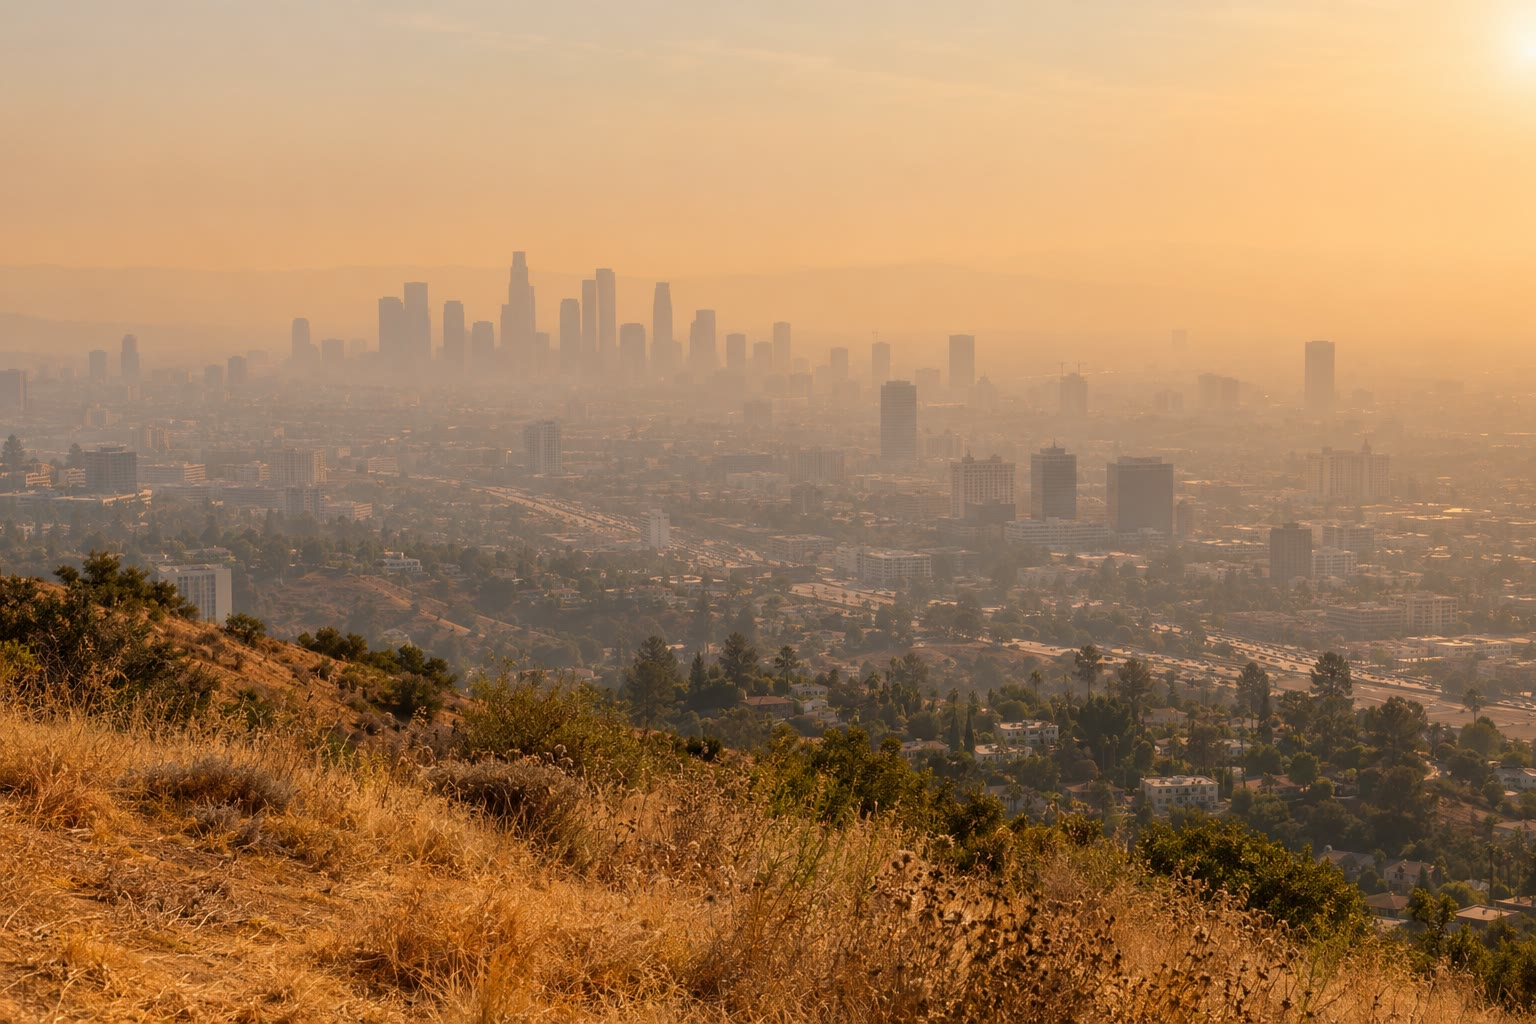
\includegraphics[width=0.6\linewidth]{images/book4/ai/b3-14-smog.jpg}

{\small एक गर्म अपराह्न में \omterm{def:b3:photochemistry:smog}{प्रकाशरासायनिक धूम-कोहरे} के नीचे एक नगर। भूरी आभा
\ce{NO2} से आती है; ओज़ोन, जो फेफड़ों को उत्तेजित करती है, अदृश्य है।}
\end{omfigure}

\begin{omfigure}
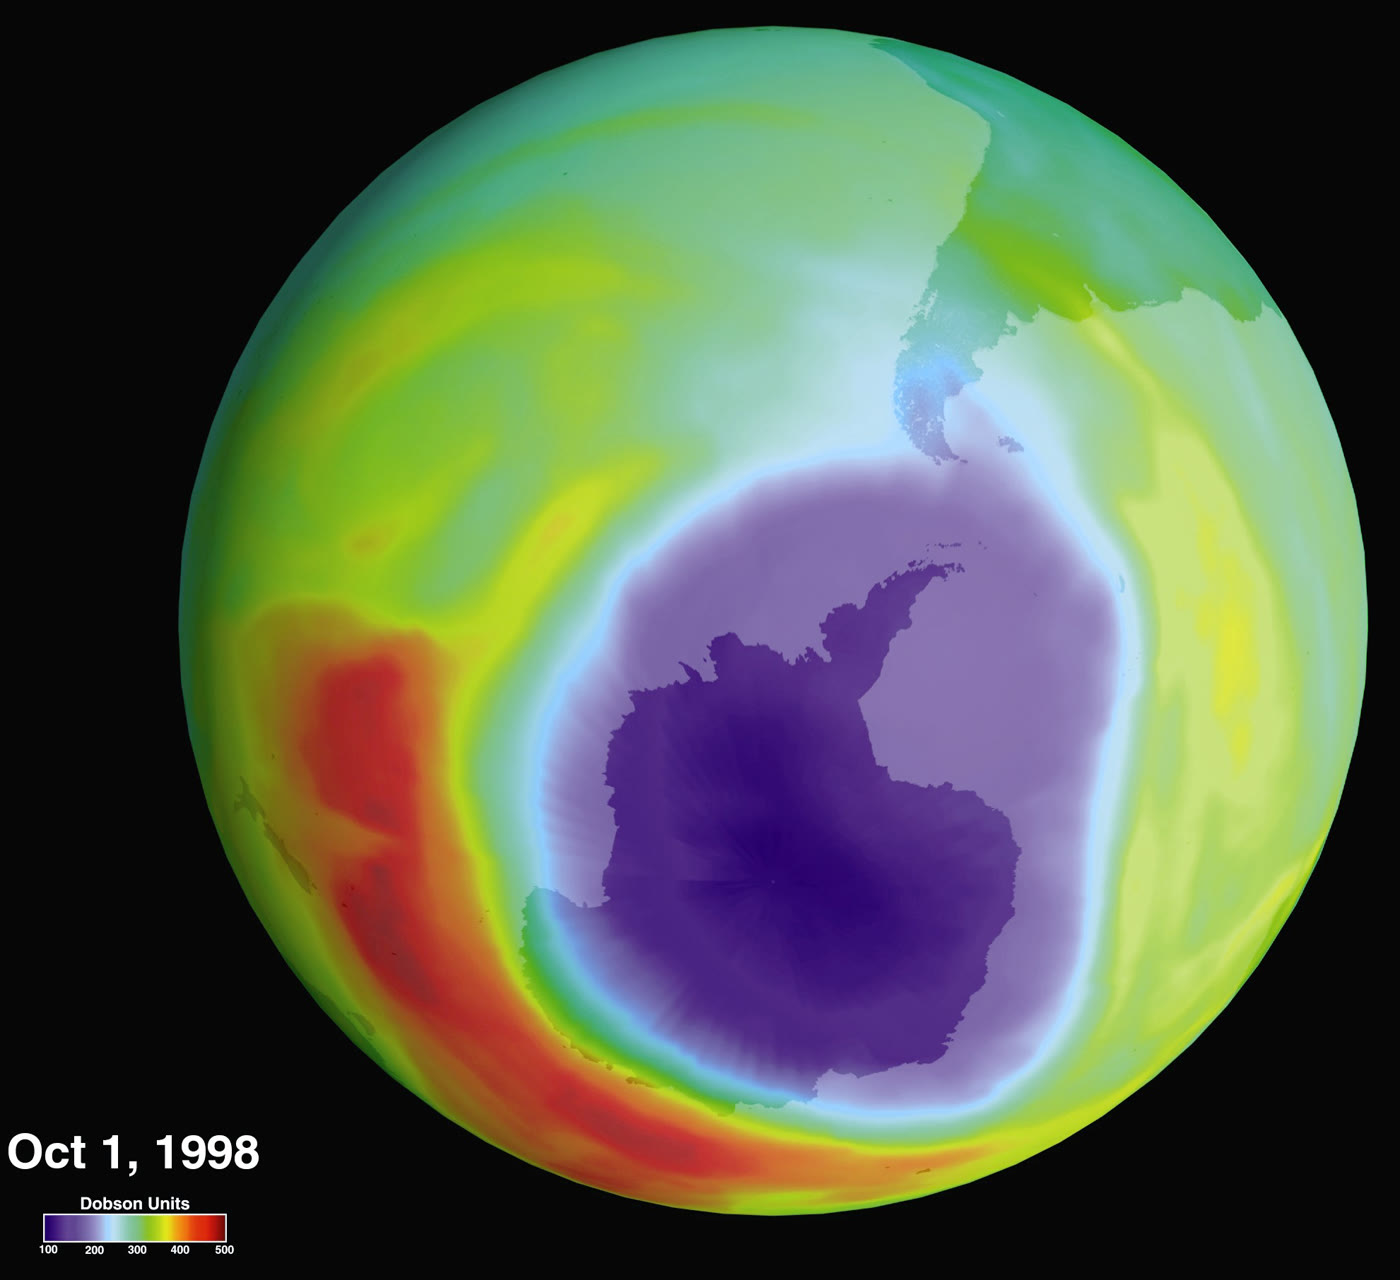
\includegraphics[width=0.5\linewidth]{images/book4/ozone-hole.jpg}

{\small 1 अक्टूबर 1998 को दक्षिणी गोलार्ध के ऊपर ओज़ोन स्तंभ, उपग्रह
मापनों से: अंटार्कटिका के ऊपर ओज़ोन छिद्र (बैंगनी) लगभग
100 डॉबसन इकाई तक गिर जाता है, जबकि अन्यत्र लगभग 300।}
\end{omfigure}

\begin{inthelab}[एक प्रकाश-रिएक्टर]
क्वार्ट्ज़ आवरण में ठंडा किया गया एक मध्यम-दाब पारा लैंप अभिक्रिया पात्र के केंद्र में
रहता है; काँच की एक फ़िल्टर आस्तीन लगभग \qty{300}{nm} से नीचे की तरंगदैर्ध्यों को हटा देती है,
जो उत्पादों को नष्ट कर देतीं। विलयन को नाइट्रोजन की धारा से
विऑक्सीजनित किया जाता है (ऑक्सीजन त्रिकों का शमन करती है) और विलोडित किया जाता है।
पूरा रिएक्टर बंद रहता है: लैंप आँखों और त्वचा के लिए हानिकारक पराबैंगनी प्रकाश
उत्सर्जित करता है, और उसे कभी नहीं देखा जाता, क्षण भर के लिए भी नहीं।
\end{inthelab}

\begin{safety}{\ghs[0.8cm]{GHS08}\ghs[0.8cm]{GHS09}}
% ledger: ghs4:benzophenone
बेंज़ोफ़ीनोन, एक सामान्य सुग्राहीकारक और प्रकाश-अपचयन का अभिकारक:
कैंसर उत्पन्न करने का संदेह, दीर्घ संपर्क के बाद अंगों को क्षति पहुँचा सकता है,
जलीय जीवन के लिए विषैला। दस्ताने पहनकर तौला और सँभाला जाता है; अवशेष
कार्बनिक अपशिष्ट में जाते हैं।
\end{safety}

\begin{history}[भविष्य का प्रकाशरसायन, और आकाश का छिद्र]
1912 में बोलोन्या में जाकोमो चामिचान ने पूछा कि क्या उद्योग एक दिन कोयले के बजाय,
पौधों की तरह, सूर्यप्रकाश पर चल सकता है; उन्होंने वर्षों तक अपनी प्रयोगशाला की छत पर
कार्बनिक यौगिकों के फ़्लास्कों को धूप में रखा था। 1985 में,
अंटार्कटिका के एक अनुसंधान केंद्र पर कार्यरत तीन वैज्ञानिकों ने बताया कि उसके ऊपर
वसंतकालीन ओज़ोन स्तंभ 1970 के दशक के उत्तरार्ध से तेज़ी से
घट रहा था।
ओज़ोन छिद्र, जिसकी व्याख्या कुछ ही वर्षों में इस अध्याय के रसायन से हो गई,
क्लोरोफ़्लुओरोकार्बनों को चरणबद्ध रूप से समाप्त करने का कारण बना।
\end{history}

\section{अभ्यास}

\begin{exercise}[$\star$]\label{exo:b3:photochemistry:1}
एक लैंप \qty{365}{nm} पर \qty{100}{mW} प्रदान करता है। प्रति सेकंड कितने फ़ोटॉन, और
प्रति सेकंड कितने आइंस्टाइन?
\end{exercise}

\begin{exercise}[$\star$]\label{exo:b3:photochemistry:2}
\qty{10.0}{min} में, \qty{1.00e-7}{einstein.s^{-1}} अवशोषित करने वाला एक विलयन
\qty{2.0e-5}{mol} अभिकारक रूपांतरित करता है। \omterm{def:b3:electronic-spectroscopy:quantum-yield}{क्वांटम लब्धि} की गणना कीजिए।
\end{exercise}

\begin{exercise}[$\star$]\label{exo:b3:photochemistry:3}
\ce{H2} की \ce{Cl2} के साथ प्रकाशरासायनिक अभिक्रिया की \omterm{def:b3:electronic-spectroscopy:quantum-yield}{क्वांटम लब्धियाँ} $10^4$ तक और
उससे अधिक होती हैं। इससे क्या पता चलता है? संचरण चरण लिखिए।
\end{exercise}

\begin{exercise}[$\star$]\label{exo:b3:photochemistry:4}
% ledger: janaf:O.dfH0, janaf:O3.dfH0
0 K पर O (\qty{246.79}{kJ/mol}) और \ce{O3}
(\qty{145.35}{kJ/mol}) की संभवन एन्थैल्पियों से, वे दीर्घतम तरंगदैर्ध्य परिकलित कीजिए जो \ce{O2} को दो
परमाणुओं में और \ce{O3} को \ce{O2} और O में विभाजित कर सकती हैं।
\end{exercise}

\begin{exercise}[$\star\star$]\label{exo:b3:photochemistry:5}
एक प्रकाश-स्विच के लिए \qty{365}{nm} पर $\varepsilon_E = 22\,000$ और $\varepsilon_Z = 1500$ \unit{L.mol^{-1}.cm^{-1}} हैं, तथा
$\Phi_{E\to Z} = 0.11$ और $\Phi_{Z\to E} = 0.40$ (अभ्यास के आँकड़े)। प्रकाशस्थायी
संघटन की गणना कीजिए।
\end{exercise}

\begin{exercise}[$\star\star$]\label{exo:b3:photochemistry:6}
हेक्सेन-2-ओन की \omterm{def:b3:photochemistry:norrish}{नॉरिश प्रकार II अभिक्रिया} के उत्पाद बताइए, और समझाइए कि
पेन्टेन-2-ओन प्रोपीन के बजाय एथीन क्यों देता है।
\end{exercise}

\begin{exercise}[$\star\star$]\label{exo:b3:photochemistry:7}
एक ग्राही की त्रिक ऊर्जा \qty{250}{kJ/mol} है। 289, 253 और \qty{236}{kJ/mol} त्रिक ऊर्जाओं वाले
तीन संभावित सुग्राहीकारकों में से (अभ्यास के आँकड़े) कौन दक्षता से स्थानांतरण करता है? प्रत्येक के
लिए \qty{298}{K} पर स्थानांतरण के साम्य स्थिरांक का आकलन कीजिए।
\end{exercise}

\begin{exercise}[$\star\star$]\label{exo:b3:photochemistry:8}
% ledger: kin:O+O2+M.k0, kin:O+O2+M.n
\qty{230}{K} पर, $[\mathrm M] = \qty{4.0e17}{cm^{-3}}$, $[\ce{O2}] = 0.21[\mathrm M]$ और $j_3 = \qty{1.0e-3}{s^{-1}}$ के साथ,
$k_2$ और स्थायी-अवस्था अनुपात $[\ce{O}]/[\ce{O3}]$ की गणना कीजिए।
\end{exercise}

\begin{exercise}[$\star\star$]\label{exo:b3:photochemistry:9}
% ledger: kin:Cl+O3.A, kin:Cl+O3.EaR, kin:Cl+CH4.A, kin:Cl+CH4.EaR
\qty{230}{K} पर $\ce{Cl + O3}$ और $\ce{Cl + CH4}$ के दर स्थिरांक परिकलित कीजिए, तथा
वह प्रायिकता कि कोई Cl परमाणु \ce{O3} से मिलता है, \ce{CH4} से नहीं, जब $[\ce{O3}] = \qty{5.7e12}{cm^{-3}}$
और $[\ce{CH4}] = \qty{4.0e11}{cm^{-3}}$।
\end{exercise}

\begin{exercise}[$\star\star\star$]\label{exo:b3:photochemistry:10}
% ledger: kin:NO+O3.A, kin:NO+O3.EaR
किसी नगर में दोपहर को $[\ce{NO2}]/[\ce{NO}] = 1.5$ और $j_{\ce{NO2}} = \qty{8.0e-3}{s^{-1}}$ हैं।
\qty{298}{K} पर प्रकाशस्थायी ओज़ोन, अणु प्रति \unit{cm^3} में और ppb में (\qty{1}{bar} पर वायु), परिकलित कीजिए।
रात में क्या होता है?
\end{exercise}

\begin{exercise}[$\star\star\star$]\label{exo:b3:photochemistry:11}
\qty{313}{nm} पर अवशोषकता 0.50 वाला एक \qty{3.0}{mL} विलयन उस तरंगदैर्ध्य पर \qty{50}{mW}
प्रकाश ग्रहण करता है; अभिक्रिया के लिए $\Phi = 0.25$। प्रारंभिक दर
\unit{mol.L^{-1}.s^{-1}} में परिकलित कीजिए।
\end{exercise}

\begin{exercise}[$\star\star\star$]\label{exo:b3:photochemistry:12}
एक फ़ेरीऑक्सैलेट प्रकाशमापी, \qty{365}{nm} पर 1.25 की \omterm{def:b3:electronic-spectroscopy:quantum-yield}{क्वांटम लब्धि} (अभ्यास के
आँकड़े) और पूर्ण अवशोषण के साथ, \qty{60}{s} में \qty{3.0e-6}{mol} Fe(II) बनाता है।
\omterm{def:b3:photochemistry:photon-flux}{फ़ोटॉन फ़्लक्स} परिकलित कीजिए। रूपांतरण कम क्यों रहना चाहिए?
\end{exercise}

\section{समस्या: ओज़ोन परत का बनना और मिटना}

\begin{problem}[{सप्ताहांत समस्या --- ओज़ोन परत का बनना और मिटना: फ़ोटॉन
देहलियाँ, मूल्यांकित दर स्थिरांकों के साथ चैपमैन स्थायी अवस्था,
क्लोरीन चक्र, और वे भंडार जो उसे रोकते हैं}]
\label{pb:b3:photochemistry:1}
% ledger: janaf:O.dfH0, janaf:O3.dfH0, kin:O+O2+M.k0, kin:O+O2+M.n, kin:O+O3.A, kin:O+O3.EaR, kin:Cl+O3.A, kin:Cl+O3.EaR, kin:O+ClO.A, kin:O+ClO.EaR, kin:Cl+CH4.A, kin:Cl+CH4.EaR, kin:ClO+NO2+M.k0, kin:ClO+NO2+M.n, kin:ClO+NO2+M.kinf, kin:ClO+NO2+M.Fc, oz:column.mean, oz:column.hole
लगभग \qty{30}{km} पर समतापमंडल का एक मॉडल (समस्या के आँकड़े): $T = \qty{230}{K}$, $[\mathrm M] =
\qty{4.0e17}{cm^{-3}}$, $[\ce{O2}] = 0.21[\mathrm M]$, \omterm{def:b3:photochemistry:photolysis}{प्रकाश-अपघटन दर स्थिरांक} $j_1 = \qty{1.0e-11}{s^{-1}}$ (\ce{O2})
और $j_3 = \qty{1.0e-3}{s^{-1}}$ (\ce{O3}), $[\ce{CH4}] = \qty{4.0e11}{cm^{-3}}$, $[\ce{NO2}] = \qty{1.0e9}{cm^{-3}}$। मूल्यांकित दर
स्थिरांक (\unit{cm^3.s^{-1}}, या $k_2$ के लिए \unit{cm^6.s^{-1}}, सांद्रताएँ प्रति \unit{cm^3} गिनी जाती हैं):
$k_2 = \num{6.0e-34}(T/300)^{-2.6}$; $k_4 = \num{8.0e-12}\eu^{-2060/T}$; Cl + \ce{O3}: $\num{2.8e-11}\eu^{-250/T}$;
O + ClO: $\num{2.5e-11}\eu^{110/T}$; Cl + \ce{CH4}: $\num{6.6e-12}\eu^{-1240/T}$; ClO + \ce{NO2} + M: $\num{1.41e-13}$,
इन परिस्थितियों में।

\medskip\noindent\textbf{भाग I --- फ़ोटॉन देहलियाँ।}
\begin{enumerate}
  \item $D_0(\ce{O2})$ परिकलित कीजिए, $\Delta_fH^\circ_0(\ce{O}) = \qty{246.79}{kJ/mol}$ से।
  \item वह दीर्घतम तरंगदैर्ध्य निकालिए जो \ce{O2} को विभाजित करती है।
  \item $\ce{O3 -> O2 + O}$ की ऊर्जा ($\Delta_fH^\circ_0(\ce{O3}) = \qty{145.35}{kJ/mol}$) और उसकी
        देहली तरंगदैर्ध्य परिकलित कीजिए।
  \item इस प्रकार दृश्य प्रकाश ओज़ोन को विभाजित कर सकता है; फिर ओज़ोन का पराबैंगनी अवशोषण
        ही जीवन के लिए महत्त्वपूर्ण क्यों है?
  \item \ce{O2} का \omterm{def:b3:photochemistry:photolysis}{प्रकाश-अपघटन} केवल वायुमंडल में ऊँचाई पर ही क्यों होता है?
\end{enumerate}

\medskip\noindent\textbf{भाग II --- चैपमैन स्थायी अवस्था।}
\begin{enumerate}[resume]
  \item चैपमैन के चारों चरण लिखिए।
  \item \qty{230}{K} पर $k_2$ और $k_2[\mathrm M]$ परिकलित कीजिए।
  \item $k_4$ परिकलित कीजिए।
  \item $[\ce{O}]/[\ce{O3}]$ परिकलित कीजिए।
  \item दिखाइए कि $[\ce{O3}] = [\ce{O2}]\sqrt{j_1k_2[\mathrm M]/(j_3k_4)}$।
  \item $[\ce{O3}]$ और उसका मिश्रण अनुपात परिकलित कीजिए।
  \item $[\ce{O}]$ परिकलित कीजिए।
  \item प्रेक्षित ओज़ोन इससे कम है। क्यों?
\end{enumerate}

\medskip\noindent\textbf{भाग III --- क्लोरीन चक्र।}
\begin{enumerate}[resume]
  \item चक्र और उसकी नेट अभिक्रिया लिखिए।
  \item \ce{O3} के विरुद्ध एक Cl परमाणु का आयुकाल परिकलित कीजिए।
  \item O के विरुद्ध ClO का आयुकाल परिकलित कीजिए।
  \item स्थायी अनुपात $[\ce{ClO}]/[\ce{Cl}]$ निकालिए।
  \item $[\ce{Cl}] + [\ce{ClO}] = \qty{1.0e7}{cm^{-3}}$ के साथ, चक्र द्वारा विषम-ऑक्सीजन ह्रास की दर की तुलना
        चैपमैन चरण $\ce{O + O3}$ की दर से कीजिए।
  \item कौन-सा चरण चक्र को सीमित करता है?
\end{enumerate}

\medskip\noindent\textbf{भाग IV --- भंडार।}
\begin{enumerate}[resume]
  \item वह प्रायिकता परिकलित कीजिए कि एक Cl परमाणु \ce{O3} से अभिक्रिया करता है,
        \ce{CH4} से नहीं।
  \item वह प्रायिकता परिकलित कीजिए कि ClO, \ce{NO2} के बजाय O से अभिक्रिया करता है।
  \item वह प्रायिकता $p$ निकालिए कि चक्र का एक चक्कर पूरा होता है।
  \item क्लोरीन के पकड़े जाने से पहले चक्करों की माध्य संख्या निकालिए।
  \item समझाइए कि ध्रुवीय समतापमंडलीय बादल शृंखला को कैसे लंबा करते हैं।
  \item परिणाम बताइए: इस मॉडल में, किसी भंडार में पकड़े जाने से पहले एक क्लोरीन परमाणु
        कितने ओज़ोन अणु नष्ट करता है।
\end{enumerate}
\end{problem}
